\documentclass[twoside]{book}

% Packages required by doxygen
\usepackage{fixltx2e}
\usepackage{calc}
\usepackage{doxygen}
\usepackage[export]{adjustbox} % also loads graphicx
\usepackage{graphicx}
\usepackage[utf8]{inputenc}
\usepackage{makeidx}
\usepackage{multicol}
\usepackage{multirow}
\PassOptionsToPackage{warn}{textcomp}
\usepackage{textcomp}
\usepackage[nointegrals]{wasysym}
\usepackage[table]{xcolor}

% Font selection
\usepackage[T1]{fontenc}
\usepackage[scaled=.90]{helvet}
\usepackage{courier}
\usepackage{amssymb}
\usepackage{sectsty}
\renewcommand{\familydefault}{\sfdefault}
\allsectionsfont{%
  \fontseries{bc}\selectfont%
  \color{darkgray}%
}
\renewcommand{\DoxyLabelFont}{%
  \fontseries{bc}\selectfont%
  \color{darkgray}%
}
\newcommand{\+}{\discretionary{\mbox{\scriptsize$\hookleftarrow$}}{}{}}

% Page & text layout
\usepackage{geometry}
\geometry{%
  a4paper,%
  top=2.5cm,%
  bottom=2.5cm,%
  left=2.5cm,%
  right=2.5cm%
}
\tolerance=750
\hfuzz=15pt
\hbadness=750
\setlength{\emergencystretch}{15pt}
\setlength{\parindent}{0cm}
\setlength{\parskip}{3ex plus 2ex minus 2ex}
\makeatletter
\renewcommand{\paragraph}{%
  \@startsection{paragraph}{4}{0ex}{-1.0ex}{1.0ex}{%
    \normalfont\normalsize\bfseries\SS@parafont%
  }%
}
\renewcommand{\subparagraph}{%
  \@startsection{subparagraph}{5}{0ex}{-1.0ex}{1.0ex}{%
    \normalfont\normalsize\bfseries\SS@subparafont%
  }%
}
\makeatother

% Headers & footers
\usepackage{fancyhdr}
\pagestyle{fancyplain}
\fancyhead[LE]{\fancyplain{}{\bfseries\thepage}}
\fancyhead[CE]{\fancyplain{}{}}
\fancyhead[RE]{\fancyplain{}{\bfseries\leftmark}}
\fancyhead[LO]{\fancyplain{}{\bfseries\rightmark}}
\fancyhead[CO]{\fancyplain{}{}}
\fancyhead[RO]{\fancyplain{}{\bfseries\thepage}}
\fancyfoot[LE]{\fancyplain{}{}}
\fancyfoot[CE]{\fancyplain{}{}}
\fancyfoot[RE]{\fancyplain{}{\bfseries\scriptsize Generated by Doxygen }}
\fancyfoot[LO]{\fancyplain{}{\bfseries\scriptsize Generated by Doxygen }}
\fancyfoot[CO]{\fancyplain{}{}}
\fancyfoot[RO]{\fancyplain{}{}}
\renewcommand{\footrulewidth}{0.4pt}
\renewcommand{\chaptermark}[1]{%
  \markboth{#1}{}%
}
\renewcommand{\sectionmark}[1]{%
  \markright{\thesection\ #1}%
}

% Indices & bibliography
\usepackage{natbib}
\usepackage[titles]{tocloft}
\setcounter{tocdepth}{3}
\setcounter{secnumdepth}{5}
\makeindex

% Hyperlinks (required, but should be loaded last)
\usepackage{ifpdf}
\ifpdf
  \usepackage[pdftex,pagebackref=true]{hyperref}
\else
  \usepackage[ps2pdf,pagebackref=true]{hyperref}
\fi
\hypersetup{%
  colorlinks=true,%
  linkcolor=blue,%
  citecolor=blue,%
  unicode%
}

% Custom commands
\newcommand{\clearemptydoublepage}{%
  \newpage{\pagestyle{empty}\cleardoublepage}%
}

\usepackage{caption}
\captionsetup{labelsep=space,justification=centering,font={bf},singlelinecheck=off,skip=4pt,position=top}

%===== C O N T E N T S =====

\begin{document}

% Titlepage & ToC
\hypersetup{pageanchor=false,
             bookmarksnumbered=true,
             pdfencoding=unicode
            }
\pagenumbering{alph}
\begin{titlepage}
\vspace*{7cm}
\begin{center}%
{\Large lib Violas Client }\\
\vspace*{1cm}
{\large Generated by Doxygen 1.8.13}\\
\end{center}
\end{titlepage}
\clearemptydoublepage
\pagenumbering{roman}
\tableofcontents
\clearemptydoublepage
\pagenumbering{arabic}
\hypersetup{pageanchor=true}

%--- Begin generated contents ---
\chapter{Class Index}
\section{Class List}
Here are the classes, structs, unions and interfaces with brief descriptions\+:\begin{DoxyCompactList}
\item\contentsline{section}{\hyperlink{structviolas_1_1_account}{violas\+::\+Account} }{\pageref{structviolas_1_1_account}}{}
\item\contentsline{section}{\hyperlink{structviolas_1_1_address_and_index}{violas\+::\+Address\+And\+Index} }{\pageref{structviolas_1_1_address_and_index}}{}
\item\contentsline{section}{\hyperlink{classviolas_1_1_client}{violas\+::\+Client} }{\pageref{classviolas_1_1_client}}{}
\item\contentsline{section}{\hyperlink{structviolas_1_1_type_tag}{violas\+::\+Type\+Tag} }{\pageref{structviolas_1_1_type_tag}}{}
\end{DoxyCompactList}

\chapter{File Index}
\doxysection{File List}
Here is a list of all documented files with brief descriptions\+:\begin{DoxyCompactList}
\item\contentsline{section}{src/ffi/\mbox{\hyperlink{client_8hpp}{client.\+hpp}} }{\pageref{client_8hpp}}{}
\end{DoxyCompactList}

\chapter{Class Documentation}
\hypertarget{structviolas_1_1_account}{}\doxysection{violas\+::Account Struct Reference}
\label{structviolas_1_1_account}\index{violas::Account@{violas::Account}}
\doxysubsection*{Public Attributes}
\begin{DoxyCompactItemize}
\item 
\mbox{\Hypertarget{structviolas_1_1_account_a1fd1a06a4abd03b20d8fe1f93268ef07}\label{structviolas_1_1_account_a1fd1a06a4abd03b20d8fe1f93268ef07}} 
Address {\bfseries address}
\item 
\mbox{\Hypertarget{structviolas_1_1_account_af315853afb5e30688b838b326a9a7601}\label{structviolas_1_1_account_af315853afb5e30688b838b326a9a7601}} 
Authentication\+Key {\bfseries auth\+\_\+key}
\item 
\mbox{\Hypertarget{structviolas_1_1_account_a09773744f6179bc742dc9b6a701e056b}\label{structviolas_1_1_account_a09773744f6179bc742dc9b6a701e056b}} 
Public\+Key {\bfseries pub\+\_\+key}
\item 
\mbox{\Hypertarget{structviolas_1_1_account_a9acc19a2ca309d6b878c97dbc4698ef6}\label{structviolas_1_1_account_a9acc19a2ca309d6b878c97dbc4698ef6}} 
uint64\+\_\+t {\bfseries sequence\+\_\+number}
\item 
\mbox{\Hypertarget{structviolas_1_1_account_afa4b79d13e690c31ef5461526732eeb8}\label{structviolas_1_1_account_afa4b79d13e690c31ef5461526732eeb8}} 
Account\+Status {\bfseries status}
\end{DoxyCompactItemize}


The documentation for this struct was generated from the following file\+:\begin{DoxyCompactItemize}
\item 
src/ffi/\mbox{\hyperlink{client_8hpp}{client.\+hpp}}\end{DoxyCompactItemize}

\hypertarget{structviolas_1_1_address_and_index}{}\doxysection{violas\+::Address\+And\+Index Struct Reference}
\label{structviolas_1_1_address_and_index}\index{violas::AddressAndIndex@{violas::AddressAndIndex}}
\doxysubsection*{Public Attributes}
\begin{DoxyCompactItemize}
\item 
\mbox{\Hypertarget{structviolas_1_1_address_and_index_ae713c0d5efc15139420bfe5451b1fede}\label{structviolas_1_1_address_and_index_ae713c0d5efc15139420bfe5451b1fede}} 
Address {\bfseries address}
\item 
\mbox{\Hypertarget{structviolas_1_1_address_and_index_a7ae0b501fcdb2e3b340f52cd90f039d9}\label{structviolas_1_1_address_and_index_a7ae0b501fcdb2e3b340f52cd90f039d9}} 
size\+\_\+t {\bfseries index}
\end{DoxyCompactItemize}


The documentation for this struct was generated from the following file\+:\begin{DoxyCompactItemize}
\item 
src/ffi/\mbox{\hyperlink{client_8hpp}{client.\+hpp}}\end{DoxyCompactItemize}

\hypertarget{classviolas_1_1_client}{}\section{violas\+:\+:Client Class Reference}
\label{classviolas_1_1_client}\index{violas\+::\+Client@{violas\+::\+Client}}
\subsection*{Public Types}
\begin{DoxyCompactItemize}
\item 
\mbox{\Hypertarget{classviolas_1_1_client_adee90625a7043bafdbb30931d564f6f4}\label{classviolas_1_1_client_adee90625a7043bafdbb30931d564f6f4}} 
enum \hyperlink{classviolas_1_1_client_adee90625a7043bafdbb30931d564f6f4}{event\+\_\+type} \{ {\bfseries sent}, 
{\bfseries received}
 \}\begin{DoxyCompactList}\small\item\em evnet type \end{DoxyCompactList}
\item 
\mbox{\Hypertarget{classviolas_1_1_client_aff66e6c69ae05d46ffb9fff703b1018f}\label{classviolas_1_1_client_aff66e6c69ae05d46ffb9fff703b1018f}} 
using {\bfseries Transaction\+Augment} = std\+::variant$<$ uint8\+\_\+t, uint64\+\_\+t, \+\_\+\+\_\+uint128\+\_\+t, Address, std\+::vector$<$ uint8\+\_\+t $>$, bool $>$
\end{DoxyCompactItemize}
\subsection*{Public Member Functions}
\begin{DoxyCompactItemize}
\item 
\mbox{\Hypertarget{classviolas_1_1_client_ae2a83172b93a647ce1261cbc049379f1}\label{classviolas_1_1_client_ae2a83172b93a647ce1261cbc049379f1}} 
virtual void {\bfseries test\+\_\+connection} ()=0
\item 
\mbox{\Hypertarget{classviolas_1_1_client_aee0abed2c8162e12f4a2e7f7445176cd}\label{classviolas_1_1_client_aee0abed2c8162e12f4a2e7f7445176cd}} 
virtual \hyperlink{structviolas_1_1_address_and_index}{Address\+And\+Index} {\bfseries create\+\_\+next\+\_\+account} (const std\+::optional$<$ Address $>$ \&address=std\+::nullopt)=0
\item 
\mbox{\Hypertarget{classviolas_1_1_client_a84b107f00acefdf7c66b1ebec3e5ff35}\label{classviolas_1_1_client_a84b107f00acefdf7c66b1ebec3e5ff35}} 
virtual std\+::vector$<$ \hyperlink{structviolas_1_1_account}{Account} $>$ {\bfseries get\+\_\+all\+\_\+accounts} ()=0
\item 
\mbox{\Hypertarget{classviolas_1_1_client_affd9f58580ee202f1e94edef655f8978}\label{classviolas_1_1_client_affd9f58580ee202f1e94edef655f8978}} 
virtual void {\bfseries create\+\_\+validator\+\_\+account} (std\+::string\+\_\+view currency\+\_\+code, const Authentication\+Key \&auth\+\_\+key, std\+::string\+\_\+view human\+\_\+name)=0
\item 
\mbox{\Hypertarget{classviolas_1_1_client_a18e71a388b3893dd0bd80169899c2901}\label{classviolas_1_1_client_a18e71a388b3893dd0bd80169899c2901}} 
virtual void {\bfseries mint\+\_\+for\+\_\+testnet} (std\+::string\+\_\+view currency\+\_\+code, const Address \&receiver, uint64\+\_\+t amount)=0
\item 
virtual void \hyperlink{classviolas_1_1_client_a03f34478845c0a740cc42fa7ac97560a}{transfer} (size\+\_\+t sender\+\_\+account\+\_\+ref\+\_\+id, const Address \&receiver\+\_\+address, std\+::string\+\_\+view currency\+\_\+code, uint64\+\_\+t amount, uint64\+\_\+t gas\+\_\+unit\+\_\+price=0, uint64\+\_\+t max\+\_\+gas\+\_\+amount=1000000, std\+::string\+\_\+view gas\+\_\+currency\+\_\+code=\char`\"{}L\+BR\char`\"{})=0
\begin{DoxyCompactList}\small\item\em transfer currency \end{DoxyCompactList}\item 
\mbox{\Hypertarget{classviolas_1_1_client_a83cf2d3e86e8cf0b1b44121022a04331}\label{classviolas_1_1_client_a83cf2d3e86e8cf0b1b44121022a04331}} 
virtual void {\bfseries allow\+\_\+custom\+\_\+script} ()=0
\item 
\mbox{\Hypertarget{classviolas_1_1_client_a23218ce437ef2bb6e73ea19fb3cdd3e1}\label{classviolas_1_1_client_a23218ce437ef2bb6e73ea19fb3cdd3e1}} 
virtual void {\bfseries allow\+\_\+publishing\+\_\+module} (bool enabled)=0
\item 
\mbox{\Hypertarget{classviolas_1_1_client_a108e8d44dfeec170bae2e87cf6135e9e}\label{classviolas_1_1_client_a108e8d44dfeec170bae2e87cf6135e9e}} 
virtual void {\bfseries publish\+\_\+module} (size\+\_\+t account\+\_\+index, std\+::string\+\_\+view module\+\_\+file\+\_\+name)=0
\item 
virtual void \hyperlink{classviolas_1_1_client_aba697ca0b8ab6aba82934ff3f04c25f1}{execute\+\_\+script} (size\+\_\+t account\+\_\+index, std\+::string\+\_\+view script\+\_\+file\+\_\+name, const std\+::vector$<$ \hyperlink{structviolas_1_1_type_tag}{Type\+Tag} $>$ \&type\+\_\+tags=\{\}, const std\+::vector$<$ Transaction\+Augment $>$ \&arguments=\{\})=0
\begin{DoxyCompactList}\small\item\em Execute script file with arguments. \end{DoxyCompactList}\item 
virtual std\+::string \hyperlink{classviolas_1_1_client_a7f4a69e73d97ed34187990fdcd9b38d1}{query\+\_\+account\+\_\+info} (const Address \&address)=0
\begin{DoxyCompactList}\small\item\em Query accout status infomation. \end{DoxyCompactList}\item 
virtual std\+::string \hyperlink{classviolas_1_1_client_aaad474fa0f89c6bbef125d12749a7c70}{query\+\_\+transaction\+\_\+info} (const Address \&address, uint64\+\_\+t seq\+\_\+number, bool is\+\_\+fetching\+\_\+event)=0
\begin{DoxyCompactList}\small\item\em Query transaction inforamtion by address and seqence number. \end{DoxyCompactList}\item 
virtual std\+::string \hyperlink{classviolas_1_1_client_aa6a3d75fbd4b3bf3c7fc3282c43398e1}{query\+\_\+transaction\+\_\+info} (uint64\+\_\+t start\+\_\+version, uint64\+\_\+t limit, bool is\+\_\+fetching\+\_\+event)=0
\begin{DoxyCompactList}\small\item\em Query transaction inforamtion by range. \end{DoxyCompactList}\item 
virtual std\+::string \hyperlink{classviolas_1_1_client_ac3ff1015d91b72c78133a5b286a3f6aa}{query\+\_\+events} (const Address \&address, \hyperlink{classviolas_1_1_client_adee90625a7043bafdbb30931d564f6f4}{event\+\_\+type} type, uint64\+\_\+t start\+\_\+version, uint64\+\_\+t limit)=0
\begin{DoxyCompactList}\small\item\em Query events. \end{DoxyCompactList}\item 
\mbox{\Hypertarget{classviolas_1_1_client_ad3644d27093e9ddb77fd69264a564b50}\label{classviolas_1_1_client_ad3644d27093e9ddb77fd69264a564b50}} 
virtual void {\bfseries publish\+\_\+curency} (std\+::string\+\_\+view currency\+\_\+code)=0
\item 
\mbox{\Hypertarget{classviolas_1_1_client_a83a763c661ef099eeefd692ebd16a323}\label{classviolas_1_1_client_a83a763c661ef099eeefd692ebd16a323}} 
virtual void {\bfseries register\+\_\+currency} (std\+::string\+\_\+view currency\+\_\+code, uint64\+\_\+t exchange\+\_\+rate\+\_\+denom, uint64\+\_\+t exchange\+\_\+rate\+\_\+num, bool is\+\_\+synthetic, uint64\+\_\+t scaling\+\_\+factor, uint64\+\_\+t fractional\+\_\+part)=0
\item 
\mbox{\Hypertarget{classviolas_1_1_client_a4fdf4a8af36c33c06f6907ac7611e6e3}\label{classviolas_1_1_client_a4fdf4a8af36c33c06f6907ac7611e6e3}} 
virtual void \hyperlink{classviolas_1_1_client_a4fdf4a8af36c33c06f6907ac7611e6e3}{add\+\_\+currency\+\_\+for\+\_\+designated\+\_\+dealer} (std\+::string\+\_\+view currency\+\_\+code, const Address \&dd\+\_\+address)=0
\begin{DoxyCompactList}\small\item\em add currency for the designated dealer account \end{DoxyCompactList}\item 
\mbox{\Hypertarget{classviolas_1_1_client_acc748841260b3eaca26ec3a2c22b5eef}\label{classviolas_1_1_client_acc748841260b3eaca26ec3a2c22b5eef}} 
virtual void \hyperlink{classviolas_1_1_client_acc748841260b3eaca26ec3a2c22b5eef}{add\+\_\+currency} (size\+\_\+t account\+\_\+index, std\+::string\+\_\+view currency\+\_\+code)=0
\begin{DoxyCompactList}\small\item\em Add a currency to current account. \end{DoxyCompactList}\item 
\mbox{\Hypertarget{classviolas_1_1_client_a7e5c7f111c7b04a3b33fd4c52c9a7abb}\label{classviolas_1_1_client_a7e5c7f111c7b04a3b33fd4c52c9a7abb}} 
virtual uint64\+\_\+t \hyperlink{classviolas_1_1_client_a7e5c7f111c7b04a3b33fd4c52c9a7abb}{get\+\_\+currency\+\_\+balance} (const Address \&address, std\+::string\+\_\+view currency\+\_\+code)=0
\begin{DoxyCompactList}\small\item\em get the balance of currency for the account address \end{DoxyCompactList}\item 
\mbox{\Hypertarget{classviolas_1_1_client_a1b50ea2c7802fd82bcc51f0c4eb642e4}\label{classviolas_1_1_client_a1b50ea2c7802fd82bcc51f0c4eb642e4}} 
virtual std\+::string \hyperlink{classviolas_1_1_client_a1b50ea2c7802fd82bcc51f0c4eb642e4}{get\+\_\+all\+\_\+currency\+\_\+info} ()=0
\begin{DoxyCompactList}\small\item\em Get all currency info. \end{DoxyCompactList}\item 
\mbox{\Hypertarget{classviolas_1_1_client_a8538c57fa4d566909c0a3c3b1bd7009f}\label{classviolas_1_1_client_a8538c57fa4d566909c0a3c3b1bd7009f}} 
virtual void \hyperlink{classviolas_1_1_client_a8538c57fa4d566909c0a3c3b1bd7009f}{mint\+\_\+currency\+\_\+for\+\_\+designated\+\_\+dealer} (std\+::string\+\_\+view currency\+\_\+code, uint64\+\_\+t sliding\+\_\+nonce, const Address \&dd\+\_\+address, uint64\+\_\+t amount, uint64\+\_\+t tier\+\_\+index)=0
\begin{DoxyCompactList}\small\item\em mint currency for dd account \end{DoxyCompactList}\item 
\mbox{\Hypertarget{classviolas_1_1_client_af09de0629e5a22ac416d4c5a9f62deee}\label{classviolas_1_1_client_af09de0629e5a22ac416d4c5a9f62deee}} 
virtual void {\bfseries create\+\_\+designated\+\_\+dealer\+\_\+account} (std\+::string\+\_\+view currency\+\_\+code, uint64\+\_\+t nonce, const Address \&new\+\_\+account\+\_\+address, const Authentication\+Key \&auth\+\_\+key, std\+::string\+\_\+view human\+\_\+name, std\+::string\+\_\+view base\+\_\+url, Public\+Key compliance\+\_\+public\+\_\+key, bool add\+\_\+all\+\_\+currencies)=0
\item 
\mbox{\Hypertarget{classviolas_1_1_client_ae0b8cd2e5d65f6cc34dc6b923fde2010}\label{classviolas_1_1_client_ae0b8cd2e5d65f6cc34dc6b923fde2010}} 
virtual void {\bfseries update\+\_\+account\+\_\+authentication\+\_\+key} (const Address \&address, const Authentication\+Key \&auth\+\_\+key)=0
\item 
\mbox{\Hypertarget{classviolas_1_1_client_a93621de71b5e1a57adf52b477c896a33}\label{classviolas_1_1_client_a93621de71b5e1a57adf52b477c896a33}} 
virtual void {\bfseries create\+\_\+parent\+\_\+vasp\+\_\+account} (std\+::string\+\_\+view currency\+\_\+code, uint64\+\_\+t nonce, const Address \&new\+\_\+account\+\_\+address, const Authentication\+Key \&auth\+\_\+key, std\+::string\+\_\+view human\+\_\+name, std\+::string\+\_\+view base\+\_\+url, Public\+Key compliance\+\_\+public\+\_\+key, bool add\+\_\+all\+\_\+currencies)=0
\item 
\mbox{\Hypertarget{classviolas_1_1_client_a2a33749f60cff385eef861b8b275da20}\label{classviolas_1_1_client_a2a33749f60cff385eef861b8b275da20}} 
virtual std\+::string {\bfseries get\+\_\+exchange\+\_\+currencies} (const Address \&address)=0
\item 
\mbox{\Hypertarget{classviolas_1_1_client_a4c9e93c5cbc079b7a7ce9827d62adb4e}\label{classviolas_1_1_client_a4c9e93c5cbc079b7a7ce9827d62adb4e}} 
virtual std\+::string {\bfseries get\+\_\+exchange\+\_\+reserves} (const Address \&address)=0
\item 
\mbox{\Hypertarget{classviolas_1_1_client_a2a76fde6b8e25e35a8f51419d4b4792d}\label{classviolas_1_1_client_a2a76fde6b8e25e35a8f51419d4b4792d}} 
virtual std\+::string {\bfseries get\+\_\+liquidity\+\_\+balance} (const Address \&address)=0
\end{DoxyCompactItemize}
\subsection*{Static Public Member Functions}
\begin{DoxyCompactItemize}
\item 
\mbox{\Hypertarget{classviolas_1_1_client_a5c99fa9be8d11bb28291e21d71e8dc8d}\label{classviolas_1_1_client_a5c99fa9be8d11bb28291e21d71e8dc8d}} 
static std\+::shared\+\_\+ptr$<$ \hyperlink{classviolas_1_1_client}{Client} $>$ {\bfseries create} (uint8\+\_\+t chain\+\_\+id, std\+::string\+\_\+view url, std\+::string\+\_\+view mint\+\_\+key, std\+::string\+\_\+view mnemonic, std\+::string\+\_\+view waypoint)
\end{DoxyCompactItemize}


\subsection{Member Function Documentation}
\mbox{\Hypertarget{classviolas_1_1_client_aba697ca0b8ab6aba82934ff3f04c25f1}\label{classviolas_1_1_client_aba697ca0b8ab6aba82934ff3f04c25f1}} 
\index{violas\+::\+Client@{violas\+::\+Client}!execute\+\_\+script@{execute\+\_\+script}}
\index{execute\+\_\+script@{execute\+\_\+script}!violas\+::\+Client@{violas\+::\+Client}}
\subsubsection{\texorpdfstring{execute\+\_\+script()}{execute\_script()}}
{\footnotesize\ttfamily virtual void violas\+::\+Client\+::execute\+\_\+script (\begin{DoxyParamCaption}\item[{size\+\_\+t}]{account\+\_\+index,  }\item[{std\+::string\+\_\+view}]{script\+\_\+file\+\_\+name,  }\item[{const std\+::vector$<$ \hyperlink{structviolas_1_1_type_tag}{Type\+Tag} $>$ \&}]{type\+\_\+tags = {\ttfamily \{\}},  }\item[{const std\+::vector$<$ Transaction\+Augment $>$ \&}]{arguments = {\ttfamily \{\}} }\end{DoxyParamCaption})\hspace{0.3cm}{\ttfamily [pure virtual]}}



Execute script file with arguments. 


\begin{DoxyParams}{Parameters}
{\em account\+\_\+index} & account index of wallet \\
\hline
{\em script\+\_\+file\+\_\+name} & script file name with path \\
\hline
{\em type\+\_\+tags} & transaction \hyperlink{structviolas_1_1_type_tag}{Type\+Tag} vector for script \\
\hline
{\em arguments} & transaction argument vector for script \\
\hline
\end{DoxyParams}
\mbox{\Hypertarget{classviolas_1_1_client_a7f4a69e73d97ed34187990fdcd9b38d1}\label{classviolas_1_1_client_a7f4a69e73d97ed34187990fdcd9b38d1}} 
\index{violas\+::\+Client@{violas\+::\+Client}!query\+\_\+account\+\_\+info@{query\+\_\+account\+\_\+info}}
\index{query\+\_\+account\+\_\+info@{query\+\_\+account\+\_\+info}!violas\+::\+Client@{violas\+::\+Client}}
\subsubsection{\texorpdfstring{query\+\_\+account\+\_\+info()}{query\_account\_info()}}
{\footnotesize\ttfamily virtual std\+::string violas\+::\+Client\+::query\+\_\+account\+\_\+info (\begin{DoxyParamCaption}\item[{const Address \&}]{address }\end{DoxyParamCaption})\hspace{0.3cm}{\ttfamily [pure virtual]}}



Query accout status infomation. 


\begin{DoxyParams}{Parameters}
{\em address} & -\/ the address of account \\
\hline
\end{DoxyParams}
\begin{DoxyReturn}{Returns}
std\+::string 
\end{DoxyReturn}
\mbox{\Hypertarget{classviolas_1_1_client_ac3ff1015d91b72c78133a5b286a3f6aa}\label{classviolas_1_1_client_ac3ff1015d91b72c78133a5b286a3f6aa}} 
\index{violas\+::\+Client@{violas\+::\+Client}!query\+\_\+events@{query\+\_\+events}}
\index{query\+\_\+events@{query\+\_\+events}!violas\+::\+Client@{violas\+::\+Client}}
\subsubsection{\texorpdfstring{query\+\_\+events()}{query\_events()}}
{\footnotesize\ttfamily virtual std\+::string violas\+::\+Client\+::query\+\_\+events (\begin{DoxyParamCaption}\item[{const Address \&}]{address,  }\item[{\hyperlink{classviolas_1_1_client_adee90625a7043bafdbb30931d564f6f4}{event\+\_\+type}}]{type,  }\item[{uint64\+\_\+t}]{start\+\_\+version,  }\item[{uint64\+\_\+t}]{limit }\end{DoxyParamCaption})\hspace{0.3cm}{\ttfamily [pure virtual]}}



Query events. 


\begin{DoxyParams}{Parameters}
{\em address} & the address of account \\
\hline
{\em type} & evnet type \\
\hline
{\em start\+\_\+version} & start version \\
\hline
{\em limit} & limit of rang, amount of queried events \\
\hline
\end{DoxyParams}
\begin{DoxyReturn}{Returns}
std\+::string with json format 
\end{DoxyReturn}
\mbox{\Hypertarget{classviolas_1_1_client_aaad474fa0f89c6bbef125d12749a7c70}\label{classviolas_1_1_client_aaad474fa0f89c6bbef125d12749a7c70}} 
\index{violas\+::\+Client@{violas\+::\+Client}!query\+\_\+transaction\+\_\+info@{query\+\_\+transaction\+\_\+info}}
\index{query\+\_\+transaction\+\_\+info@{query\+\_\+transaction\+\_\+info}!violas\+::\+Client@{violas\+::\+Client}}
\subsubsection{\texorpdfstring{query\+\_\+transaction\+\_\+info()}{query\_transaction\_info()}\hspace{0.1cm}{\footnotesize\ttfamily [1/2]}}
{\footnotesize\ttfamily virtual std\+::string violas\+::\+Client\+::query\+\_\+transaction\+\_\+info (\begin{DoxyParamCaption}\item[{const Address \&}]{address,  }\item[{uint64\+\_\+t}]{seq\+\_\+number,  }\item[{bool}]{is\+\_\+fetching\+\_\+event }\end{DoxyParamCaption})\hspace{0.3cm}{\ttfamily [pure virtual]}}



Query transaction inforamtion by address and seqence number. 


\begin{DoxyParams}{Parameters}
{\em address} & the address of account \\
\hline
{\em seq\+\_\+number} & the sequence number of account \\
\hline
{\em is\+\_\+fetching\+\_\+event} & whether fectching event or not \\
\hline
\end{DoxyParams}
\begin{DoxyReturn}{Returns}
std\+::string with json format 
\end{DoxyReturn}
\mbox{\Hypertarget{classviolas_1_1_client_aa6a3d75fbd4b3bf3c7fc3282c43398e1}\label{classviolas_1_1_client_aa6a3d75fbd4b3bf3c7fc3282c43398e1}} 
\index{violas\+::\+Client@{violas\+::\+Client}!query\+\_\+transaction\+\_\+info@{query\+\_\+transaction\+\_\+info}}
\index{query\+\_\+transaction\+\_\+info@{query\+\_\+transaction\+\_\+info}!violas\+::\+Client@{violas\+::\+Client}}
\subsubsection{\texorpdfstring{query\+\_\+transaction\+\_\+info()}{query\_transaction\_info()}\hspace{0.1cm}{\footnotesize\ttfamily [2/2]}}
{\footnotesize\ttfamily virtual std\+::string violas\+::\+Client\+::query\+\_\+transaction\+\_\+info (\begin{DoxyParamCaption}\item[{uint64\+\_\+t}]{start\+\_\+version,  }\item[{uint64\+\_\+t}]{limit,  }\item[{bool}]{is\+\_\+fetching\+\_\+event }\end{DoxyParamCaption})\hspace{0.3cm}{\ttfamily [pure virtual]}}



Query transaction inforamtion by range. 


\begin{DoxyParams}{Parameters}
{\em start\+\_\+version} & start version \\
\hline
{\em limit} & limit of range, amount of queried transaction \\
\hline
{\em is\+\_\+fetching\+\_\+event} & whether fectching event or not \\
\hline
\end{DoxyParams}
\begin{DoxyReturn}{Returns}
std\+::string with json format 
\end{DoxyReturn}
\mbox{\Hypertarget{classviolas_1_1_client_a03f34478845c0a740cc42fa7ac97560a}\label{classviolas_1_1_client_a03f34478845c0a740cc42fa7ac97560a}} 
\index{violas\+::\+Client@{violas\+::\+Client}!transfer@{transfer}}
\index{transfer@{transfer}!violas\+::\+Client@{violas\+::\+Client}}
\subsubsection{\texorpdfstring{transfer()}{transfer()}}
{\footnotesize\ttfamily virtual void violas\+::\+Client\+::transfer (\begin{DoxyParamCaption}\item[{size\+\_\+t}]{sender\+\_\+account\+\_\+ref\+\_\+id,  }\item[{const Address \&}]{receiver\+\_\+address,  }\item[{std\+::string\+\_\+view}]{currency\+\_\+code,  }\item[{uint64\+\_\+t}]{amount,  }\item[{uint64\+\_\+t}]{gas\+\_\+unit\+\_\+price = {\ttfamily 0},  }\item[{uint64\+\_\+t}]{max\+\_\+gas\+\_\+amount = {\ttfamily 1000000},  }\item[{std\+::string\+\_\+view}]{gas\+\_\+currency\+\_\+code = {\ttfamily \char`\"{}LBR\char`\"{}} }\end{DoxyParamCaption})\hspace{0.3cm}{\ttfamily [pure virtual]}}



transfer currency 


\begin{DoxyParams}{Parameters}
{\em sender\+\_\+account\+\_\+ref\+\_\+id} & the account index of client\textquotesingle{}s wallet \\
\hline
{\em receiver\+\_\+address} & the address of receiver \\
\hline
{\em currency\+\_\+code} & currency code \\
\hline
{\em amount} & the amount of currency \\
\hline
{\em gas\+\_\+unit\+\_\+price} & the gas unit price \\
\hline
{\em max\+\_\+gas\+\_\+amount} & the max gas amount, default is 1,000,000 \\
\hline
{\em gas\+\_\+currency\+\_\+code} & the gas currency code. default is \textquotesingle{}L\+BR\textquotesingle{} \\
\hline
\end{DoxyParams}


The documentation for this class was generated from the following file\+:\begin{DoxyCompactItemize}
\item 
/home/hunter/\+Projects/work/\+Violas\+Client\+Sdk/rust/client-\/proxy/src/ffi/\hyperlink{client_8hpp}{client.\+hpp}\end{DoxyCompactItemize}

\hypertarget{structviolas_1_1_type_tag}{}\section{violas\+:\+:Type\+Tag Struct Reference}
\label{structviolas_1_1_type_tag}\index{violas\+::\+Type\+Tag@{violas\+::\+Type\+Tag}}
\subsection*{Public Member Functions}
\begin{DoxyCompactItemize}
\item 
\mbox{\Hypertarget{structviolas_1_1_type_tag_ad0b02cd93f45bceaf8316657f7576e04}\label{structviolas_1_1_type_tag_ad0b02cd93f45bceaf8316657f7576e04}} 
{\bfseries Type\+Tag} (Address addr, std\+::string\+\_\+view mod, std\+::string\+\_\+view res)
\item 
\mbox{\Hypertarget{structviolas_1_1_type_tag_a24d765f5fdad075cf6e1b4e1d72b7509}\label{structviolas_1_1_type_tag_a24d765f5fdad075cf6e1b4e1d72b7509}} 
{\bfseries Type\+Tag} (const \hyperlink{structviolas_1_1_type_tag}{Type\+Tag} \&tag)
\item 
\mbox{\Hypertarget{structviolas_1_1_type_tag_acd039f4d463a0bf2b7627ceac0f8fb8e}\label{structviolas_1_1_type_tag_acd039f4d463a0bf2b7627ceac0f8fb8e}} 
{\bfseries Type\+Tag} (\hyperlink{structviolas_1_1_type_tag}{Type\+Tag} \&\&tag)
\item 
\mbox{\Hypertarget{structviolas_1_1_type_tag_a6fad44c67023475d91031d6ea7c96a50}\label{structviolas_1_1_type_tag_a6fad44c67023475d91031d6ea7c96a50}} 
\hyperlink{structviolas_1_1_type_tag}{Type\+Tag} \& {\bfseries operator=} (\hyperlink{structviolas_1_1_type_tag}{Type\+Tag} \&\&tag)
\end{DoxyCompactItemize}
\subsection*{Public Attributes}
\begin{DoxyCompactItemize}
\item 
\mbox{\Hypertarget{structviolas_1_1_type_tag_acc653128cb55dca87509c003416d49c4}\label{structviolas_1_1_type_tag_acc653128cb55dca87509c003416d49c4}} 
Address {\bfseries address}
\item 
\mbox{\Hypertarget{structviolas_1_1_type_tag_a460ac5aba207c2c0285ed567b26788cd}\label{structviolas_1_1_type_tag_a460ac5aba207c2c0285ed567b26788cd}} 
std\+::string {\bfseries module\+\_\+name}
\item 
\mbox{\Hypertarget{structviolas_1_1_type_tag_a39c0e6e421373e2eb8e4180064cb510b}\label{structviolas_1_1_type_tag_a39c0e6e421373e2eb8e4180064cb510b}} 
std\+::string {\bfseries resource\+\_\+name}
\end{DoxyCompactItemize}


The documentation for this struct was generated from the following file\+:\begin{DoxyCompactItemize}
\item 
/home/hunter/\+Projects/work/\+Violas\+Client\+Sdk/rust/client-\/proxy/src/ffi/\hyperlink{client_8hpp}{client.\+hpp}\end{DoxyCompactItemize}

\chapter{File Documentation}
\hypertarget{client_8hpp}{}\doxysection{src/ffi/client.hpp File Reference}
\label{client_8hpp}\index{src/ffi/client.hpp@{src/ffi/client.hpp}}
{\ttfamily \#include $<$memory$>$}\newline
{\ttfamily \#include $<$array$>$}\newline
{\ttfamily \#include $<$vector$>$}\newline
{\ttfamily \#include $<$string$>$}\newline
{\ttfamily \#include $<$string\+\_\+view$>$}\newline
{\ttfamily \#include $<$limits$>$}\newline
{\ttfamily \#include $<$variant$>$}\newline
{\ttfamily \#include $<$optional$>$}\newline
Include dependency graph for client.\+hpp\+:
\nopagebreak
\begin{figure}[H]
\begin{center}
\leavevmode
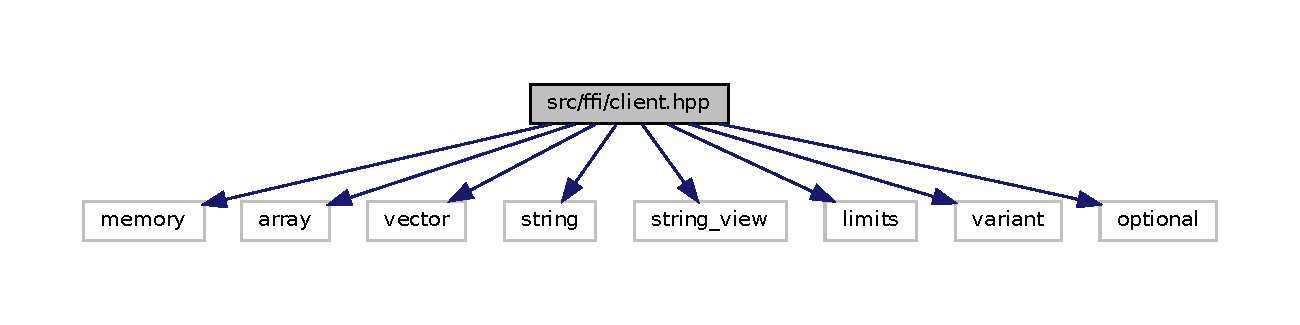
\includegraphics[width=350pt]{client_8hpp__incl}
\end{center}
\end{figure}
\doxysubsection*{Classes}
\begin{DoxyCompactItemize}
\item 
struct \mbox{\hyperlink{structviolas_1_1_address_and_index}{violas\+::\+Address\+And\+Index}}
\item 
struct \mbox{\hyperlink{structviolas_1_1_account}{violas\+::\+Account}}
\item 
struct \mbox{\hyperlink{structviolas_1_1_type_tag}{violas\+::\+Type\+Tag}}
\item 
class \mbox{\hyperlink{classviolas_1_1_client}{violas\+::\+Client}}
\end{DoxyCompactItemize}
\doxysubsection*{Typedefs}
\begin{DoxyCompactItemize}
\item 
\mbox{\Hypertarget{client_8hpp_ac4f9020df5073f2d5f031c1d3aa46ced}\label{client_8hpp_ac4f9020df5073f2d5f031c1d3aa46ced}} 
using {\bfseries violas\+::\+Address} = std\+::array$<$ uint8\+\_\+t, A\+D\+D\+R\+E\+S\+S\+\_\+\+L\+E\+N\+G\+TH $>$
\item 
\mbox{\Hypertarget{client_8hpp_a3e1e6e14f4e9fc4e11151db2da38ee19}\label{client_8hpp_a3e1e6e14f4e9fc4e11151db2da38ee19}} 
using {\bfseries violas\+::\+Authentication\+Key} = std\+::array$<$ uint8\+\_\+t, A\+D\+D\+R\+E\+S\+S\+\_\+\+L\+E\+N\+G\+TH $\ast$2 $>$
\item 
\mbox{\Hypertarget{client_8hpp_ac4cb602d427e8b018aae8704d2c9877e}\label{client_8hpp_ac4cb602d427e8b018aae8704d2c9877e}} 
using {\bfseries violas\+::\+Public\+Key} = std\+::array$<$ uint8\+\_\+t, A\+D\+D\+R\+E\+S\+S\+\_\+\+L\+E\+N\+G\+TH $\ast$2 $>$
\item 
\mbox{\Hypertarget{client_8hpp_aadbb99e13cd5b3b6afd00cfbfa337689}\label{client_8hpp_aadbb99e13cd5b3b6afd00cfbfa337689}} 
using {\bfseries violas\+::\+Vec\+U8} = std\+::vector$<$ uint8\+\_\+t $>$
\item 
\mbox{\Hypertarget{client_8hpp_abe3ebdaf7fcffbeea777de9a46f21592}\label{client_8hpp_abe3ebdaf7fcffbeea777de9a46f21592}} 
using {\bfseries violas\+::client\+\_\+ptr} = std\+::shared\+\_\+ptr$<$ Client $>$
\end{DoxyCompactItemize}
\doxysubsection*{Enumerations}
\begin{DoxyCompactItemize}
\item 
\mbox{\Hypertarget{client_8hpp_a2816db4e1fa87bb94fda0bd01a0a630e}\label{client_8hpp_a2816db4e1fa87bb94fda0bd01a0a630e}} 
enum {\bfseries Account\+Status} \{ {\bfseries Local}, 
{\bfseries Persisted}, 
{\bfseries Unknow}
 \}
\end{DoxyCompactItemize}
\doxysubsection*{Functions}
\begin{DoxyCompactItemize}
\item 
\mbox{\Hypertarget{client_8hpp_aa3784925591dd3259180f6cbb0cfafea}\label{client_8hpp_aa3784925591dd3259180f6cbb0cfafea}} 
Type\+Tag {\bfseries violas\+::make\+\_\+currency\+\_\+tag} (std\+::string\+\_\+view currency\+\_\+code)
\end{DoxyCompactItemize}
\doxysubsection*{Variables}
\begin{DoxyCompactItemize}
\item 
\mbox{\Hypertarget{client_8hpp_a97b7bdfcf727ae2d2bb13cbca3d20ba5}\label{client_8hpp_a97b7bdfcf727ae2d2bb13cbca3d20ba5}} 
const size\+\_\+t {\bfseries violas\+::\+A\+D\+D\+R\+E\+S\+S\+\_\+\+L\+E\+N\+G\+TH} = 16
\item 
\mbox{\Hypertarget{client_8hpp_a2ea6c6cd760643ef27f8c63a0cee9471}\label{client_8hpp_a2ea6c6cd760643ef27f8c63a0cee9471}} 
const uint64\+\_\+t {\bfseries violas\+::\+M\+I\+C\+R\+O\+\_\+\+C\+O\+IN} = 1E+6
\item 
\mbox{\Hypertarget{client_8hpp_aef8663b2a3c6d317f101baede32ba7ae}\label{client_8hpp_aef8663b2a3c6d317f101baede32ba7ae}} 
const uint64\+\_\+t {\bfseries violas\+::\+A\+S\+S\+O\+C\+I\+A\+T\+I\+O\+N\+\_\+\+ID} = std\+::numeric\+\_\+limits$<$uint64\+\_\+t$>$\+::max()
\item 
\mbox{\Hypertarget{client_8hpp_a2accd0e309777da7d39aec6eadf07f51}\label{client_8hpp_a2accd0e309777da7d39aec6eadf07f51}} 
const Address {\bfseries violas\+::\+A\+S\+S\+O\+C\+I\+A\+T\+I\+O\+N\+\_\+\+A\+D\+D\+R\+E\+SS} = \{00, 00, 00, 00, 00, 00, 00, 00, 00, 00, 00, 00, 0x0A, 0x55, 0x0C, 0x18\}
\item 
\mbox{\Hypertarget{client_8hpp_aac6eccd45b7f8a843b399689b2c0e08e}\label{client_8hpp_aac6eccd45b7f8a843b399689b2c0e08e}} 
const Address {\bfseries violas\+::\+T\+E\+S\+T\+N\+E\+T\+\_\+\+D\+D\+\_\+\+A\+D\+D\+R\+E\+SS} = \{00, 00, 00, 00, 00, 00, 00, 00, 00, 00, 00, 00, 00, 00, 00, 0x\+DD\}
\item 
\mbox{\Hypertarget{client_8hpp_a8fb887c3d55f75dd84c3487fbc1aa7be}\label{client_8hpp_a8fb887c3d55f75dd84c3487fbc1aa7be}} 
const Address {\bfseries violas\+::\+C\+O\+R\+E\+\_\+\+C\+O\+D\+E\+\_\+\+A\+D\+D\+R\+E\+SS} = \{00, 00, 00, 00, 00, 00, 00, 00, 00, 00, 00, 00, 00, 00, 00, 0x01\}
\end{DoxyCompactItemize}


\doxysubsection{Detailed Description}
\begin{DoxyAuthor}{Author}
Hunter Sun (\href{mailto:HunterSun2018@gmail.com}{\texttt{ Hunter\+Sun2018@gmail.\+com}}) 
\end{DoxyAuthor}
\begin{DoxyVersion}{Version}
0.\+1 
\end{DoxyVersion}
\begin{DoxyDate}{Date}
2020-\/09-\/17
\end{DoxyDate}
\begin{DoxyCopyright}{Copyright}
Copyright (c) 2020 
\end{DoxyCopyright}

%--- End generated contents ---

% Index
\backmatter
\newpage
\phantomsection
\clearemptydoublepage
\addcontentsline{toc}{chapter}{Index}
\printindex

\end{document}
